% Condition B (Pure Taxonomy) - Mechanism Hierarchy
\begin{figure}[H]
\centering
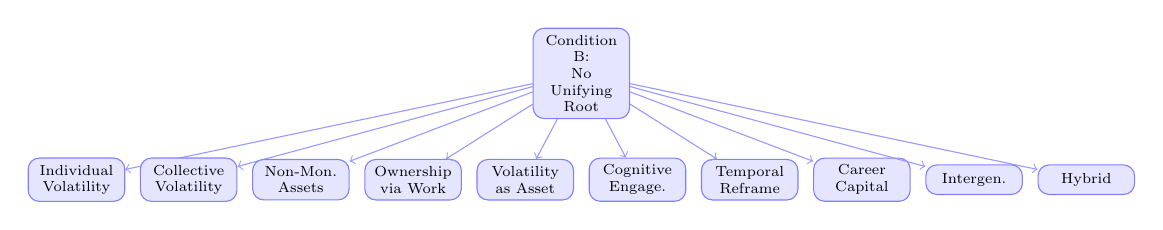
\begin{tikzpicture}[scale=0.75, transform shape,
  grow=south,
  level 1/.style={sibling distance=1.9cm, level distance=1.8cm},
  every node/.style={rectangle, rounded corners, draw=blue!50, fill=blue!10, font=\scriptsize, align=center, text width=1.4cm, minimum height=0.5cm},
  edge from parent/.style={draw, blue!40, ->},
]
\node {Condition B:\\No Unifying\\Root}
  child {node {Individual\\Volatility}}
  child {node {Collective\\Volatility}}
  child {node {Non-Mon.\\Assets}}
  child {node {Ownership\\via Work}}
  child {node {Volatility\\as Asset}}
  child {node {Cognitive\\Engage.}}
  child {node {Temporal\\Reframe}}
  child {node {Career\\Capital}}
  child {node {Intergen.}}
  child {node {Hybrid}}
;
\end{tikzpicture}
\caption{Condition B mechanism-tree schematic. Ten independent mechanism roots are shown beneath a synthetic super-root; solution nodes, candidate-to-mechanism links, and lower mechanism branches are omitted. The stored hierarchy organizes proposals around domain concepts including volatility, non-monetary assets, work-based ownership, and temporal reframing.}
\label{fig:tree-b}
\end{figure}
